\part{Step Counter Algorithm}

    \chapter{Overview}

        This section covers the development and evaluation of the step counter algorithm. The algorithm aims to extract the occurences of steps from the raw accelerometer data recorded on a smartphone. Effectively, the problem is one of peak detection in a noisy signal.

        The algorithm developed for this project was adapted from the windowed peak detection algorithm described by Palshakir \cite{palshikar}.

        The algorithm is split into five stages, each responsible for a particular function. The data flows from left to right in Figure \ref{img_sc_block} below. All stages have an input data stream and an output data stream, with the exception of the final stage. Each of the five stages will be described in detail in the following sections. Note that throughout the description there will be options or parameters for each stage; this is intentional, as this allows optimization routines to be run on the algorithm to determine the best set of parameters for overall performance. 

        \begin{figure}[h]
            \includegraphics[width=\textwidth]{Images/step_counter_block.png}
            \centering
            \caption{Block diagram of the step counter algorithm.}
            \label{img_sc_block}
        \end{figure}

    \chapter{Algorithm Description}

        \section{Pre-Processing Stage}

            The Pre-Processing Stage is responsible for two functions:

            \begin{enumerate}
                \item Formatting the data received from the accelerometer into a usable format.
                \item Ensuring a constant sampling frequency by means of linear interpolation.
            \end{enumerate}

            The project uses a tri-axial accelerometer, however the step-counting algorithm is concerned with the magnitude rather than any single directional component because the physical orientation of the device is unknown. The time stamps of the samples should also be adjusted appropriately so that the first sample received from the user initiating the algorithm is at $t = 0$. The time stamps are provided in nanoseconds and are not given in standard UTC format, but as the time since system boot. The equations for these operations are simple and are as follows:

            \begin{equation}
                m = \sqrt{a_{x}^2 + a_{y}^2 + a_{z}^2},
            \end{equation}

            \begin{equation}
                t_{i,adjusted} = \frac{t_i - t_0}{t_s},
            \end{equation}

            where $m$ is the magnitude of the acceleration signal, $a_{x}$ is the acceleration in the x direction, $a_{y}$ is the acceleration in the y direction, $a_{z}$ is the acceleration in the z direction, $t_{i,adjusted}$ is the adjusted time stamp for the i-th sample, $t_i$ is the time stamp for the i-th sample, $t_0$ is the time stamp of the initial sample, and $t_s$ is the time-scaling factor. For example, converting from nanoseconds to milliseconds, $t_s = 10^6$. 

            Each sample from the accelerometer is then inserted into a simple data structure and is appended to an internal buffer of size 2. When this buffer is full, the two points ihe buffer are linearly interpolated. Although the developer can specify a desired sample rate for the accelerometer, there is no guarantee that the accelerometer will be sampled at this rate, hence interpolation is needed. An example of this is shown below in Figure \ref{img_sampling_freq} where time between samples is plotted against samples. For the subsequent filtering stage, we need to ensure that the data is sampled at a constant rate.

            The algorithm knows what The desired sample rate determines the values of the linear interpolation equation below:

            \begin{equation}
                value = \frac{y_1 - y_0}{t_1 - t_0} t_{int} + y_0,
            \end{equation}

            where the two points of the original data stream are given by: $(t_1, y_1)$ and $(t_0, y_0)$, and the time between each equally sampled value is given by $t_{int}$.

            \begin{figure}[h]
                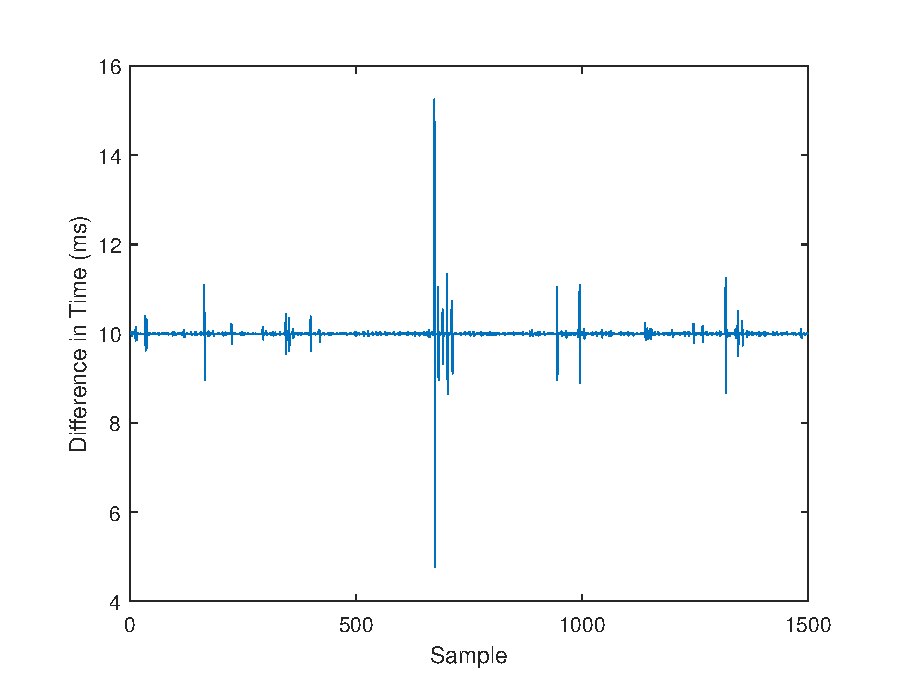
\includegraphics[width=\textwidth]{Images/sampling_freq.eps}
                \centering
                \caption{Time differences between samples for a 100Hz sampled signal. Note that the non-constant sampling times leads to the requirement for interpolation.}
                \label{img_sampling_freq}
            \end{figure}

        \section{Filtering Stage}

            The function of the filtering stage is to smooth the signal by removing as much of the high frequency noise from the accelerometer time series as possible.

            The filter required is a simple finite impulse response (FIR), low-pass digital filter. In order to capture a variety of walking speeds, the cutoff frequency for this filter will be around 3 Hz. This should be sufficient to capture the walking of even the speediest walkers, as this would translate to an pace of $5.4 mph$ according to the ratio of $2000 steps = 1 mile$ as given by the American College of Sports Medicine \cite{acsm}. Note that the average walking pace for pedestrians aged 14 to 64 was found to be $3.1 mph$ in a study by Knoblauch, et. al. \cite{walking_speed}.

            An example of the raw accelerometer signal (after interpolation) and the filtered signal is shown below in Figure \ref{img_filtered_signal}.

            \begin{figure}[h]
                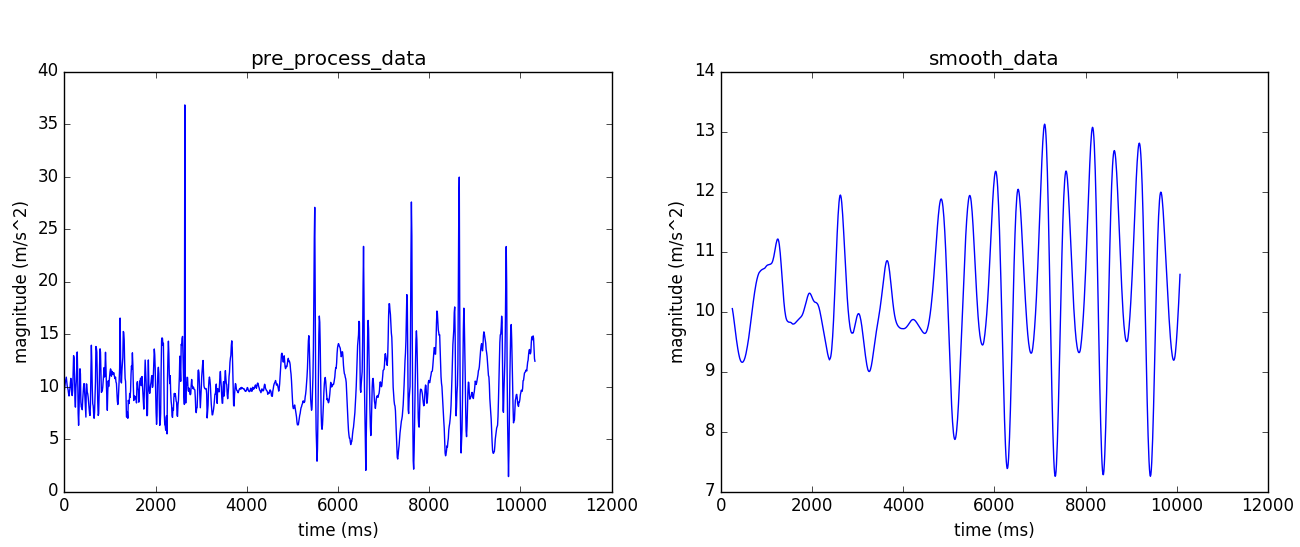
\includegraphics[width=\textwidth]{Images/filtered_signal.png}
                \centering
                \caption{Example of a signal being filtered. Filter used: Gaussian Filter with $N=51$ and $\sigma=0.35$. Note the large peaks due to noise are filtered out entirely around t = 2300ms, 5500ms, 6500ms, 7750ms, and 9750ms.}
                \label{img_filtered_signal}
            \end{figure}

            A number of filters were implemented for performance testing.

            \subsection{Moving Average}

                This is a very simple filter, each point in the filter window being weighted equally such that:

                \begin{equation}
                    m_k = \frac{1}{N},
                \end{equation}

                where $m_k$ is the $k^{th}$ filter coefficient, and $N$ is the length of the filter. The frequency response of this filter is shown below in Figure \ref{img_compare_filters}.

            \subsection{Gaussian Filter}

                This is a more complex filter, using a Gaussian as the filter coefficients. This filter attempts to suppress the sidelobes of the moving-average filter by having a smoother transition to the stop-band. The weights of the filter are given by:

                \begin{equation}
                    g_k = \exp(-\frac{1}{2}(\frac{k - \frac{N-1}{2}}{\sigma \frac{N-1}{2}})^2),
                \end{equation}

                where $g_k$ is the $k^{th}$ coefficient of the filter, $N$ is the length of the filter window, and $\sigma$ is a parameter defining the standard deviation of the Gaussian. Note that the standard deviation also scales with the length of the filter. The frequency response of this filter is shown below in Figure \ref{img_compare_filters}.

            \subsection{Hann Filter}

                This is a similar filter the Gaussian filter, which also attempts to smooth out the response by suppressing the sidelobes of the moving-average filter. The weights of the filter are derived from the Hann window [CIT] and are as follows: 

                \begin{equation}
                    h_k = \frac{1}{2}(1 - \cos(\frac{2\pi k}{N - 1}))
                \end{equation}

                where $h_k$ is the $k^{th}$ filter coefficient and $N$ is the length of the filter window. The frequency response of this filter is shown below in Figure \ref{img_compare_filters}. 

            \subsection{Kaiser-Bessel Filter}

                This is the most complex filter design, which combines the ideal filter response (note a sinc function in the time domain) and a Bessel window to achieve the desired response. The calculation of the coeffcients is as follows \cite{kaiser-bessel}:

                First, calculate the window shape parameter $\alpha$. 

                \begin{equation}
                    \alpha = 
                        \begin{cases}
                            0.1102(A - 8.7) & A \ge 50 \\
                            0.5842(A-21)^{0.4} + 0.07886(A-21) & 21 \leq A \geq 50 \\
                            0 & A \le 21
                        \end{cases},
                \end{equation}

                where $A$ is the desired attenuation at the cutoff frequency.

                Then calculate the coefficients of the Kaiser-Bessel window:

                \begin{equation}
                w_k = \frac{I_0(\alpha \sqrt{1 - (\frac{k - N_p}{N_p})^2})}{I_0(\alpha)},
                \end{equation}

                where $w_k$ is the $k^{th}$ coefficient of the window, $\alpha$ is the window shape parameter, $N_p$ is the midpoint of the filter, $N_p = \frac{N-1}{2}$ where $N$ is the length of the filter, and $I_0$ is the $0^{th}$ order Bessel function of the first kind.

                Then calculate the coefficients of the ideal filter response:

                \begin{equation}
                i_k = \frac{\sin(2\pi k\frac{F_c}{F_s})}{\pi k},
                \end{equation}

                where $i_k$ is the $k^{th}$ coefficient of the ideal filter response, $F_c$ is the desired cutoff frequency and $F_s$ is the sampling frequency.

                Finally, compute the coefficients of the filter with: 

                \begin{equation}
                b_k = w_ki_k,
                \end{equation}

                where $b_k$ is the $k^{th}$ coefficient of the Kaiser-Bessel filter response. The frequency response of this filter is shown below in Figure \ref{img_compare_filters}.

                \begin{figure}[!th]
                    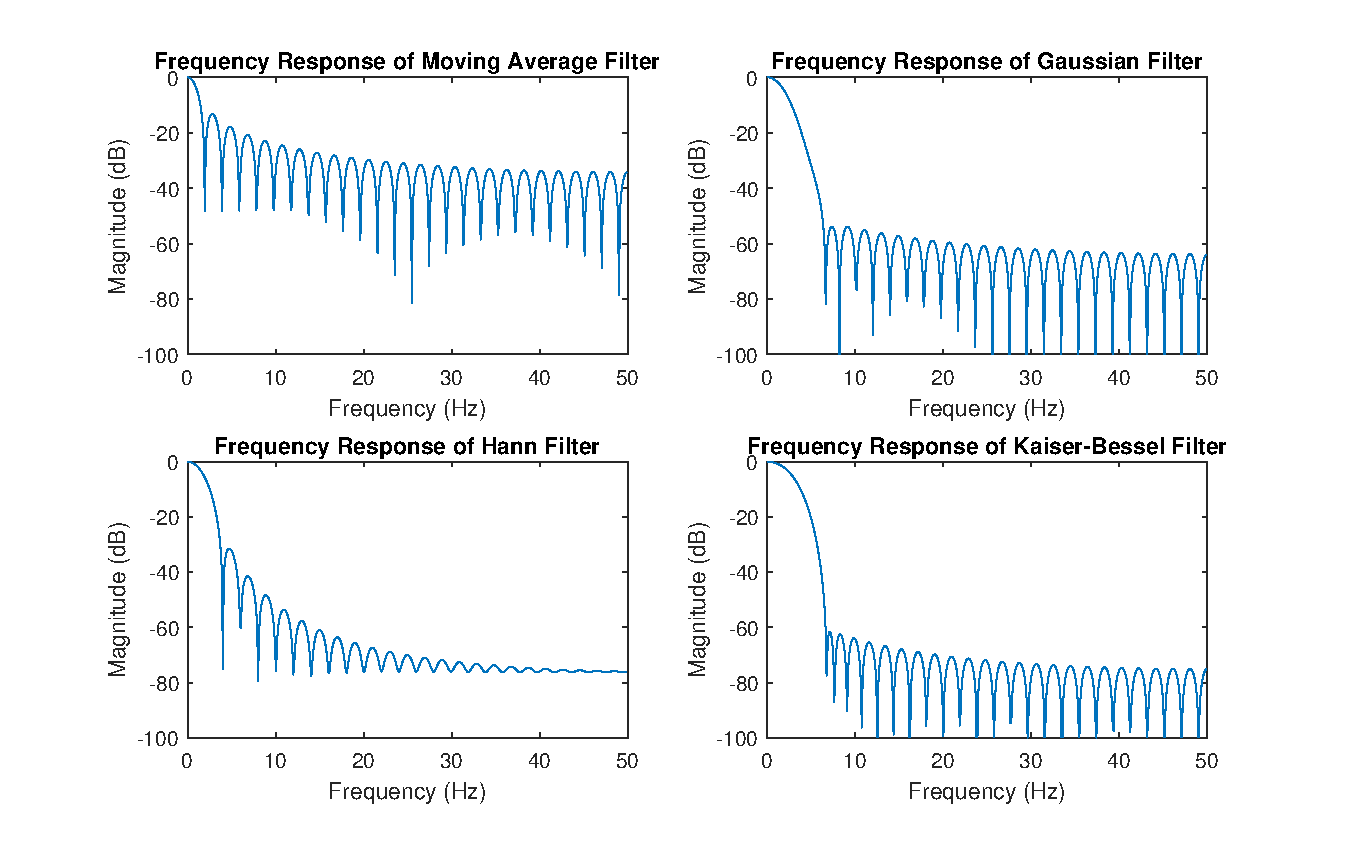
\includegraphics[width=\textwidth]{Images/compare_filters.eps}
                    \centering
                    \caption{Frequency response of the four filters compared. Starting at top-left, working clockwise: Moving Average filter with $N=51$, Gaussian filter with $N=51$ and $\sigma=0.35$, Kaiser-Bessel filter with $N=51$, $A=60dB$, $F_c = 3Hz$, and $F_s= 100Hz$, and Hann filter with $N=51$}
                    \label{img_compare_filters}
                \end{figure}  

        \section{Scoring Stage}

            The function of the scoring stage is to evaluate the 'peakiness' of given point. The result of this stage should increase the magnitude of any peak, making them more obvious to the subsequent peak detector.

            A few methods were evaluated. These are detailed below.

            \subsection{Maximum Difference}

                This method uses the local neighbours of the point in question to determine how peaky the point is. It considers the $N$ points to the left and determines the maximum difference between the point in question and those points. It does the same for the $N$ points to the right, and then averages the two maximum differences as the result.

                This operation results in enhanced peaks. An example of the output from the scoring stage using Maximum Difference is shown below in Figure \ref{img_compare_scoring}.

                The equation describing this behaviour is given by:

                \begin{equation}
                x = \frac{\max\limits_k{(x_i - x_{i-k})} + \max\limits_k{(x_i - x_{i+k})}}{2},
                \end{equation}

                where $i$ is the point under consideration, and $x_n$ is the value of the signal at the $n^{th}$ sample.
              

            \subsection{Mean Difference}

                This method is similar to the Maximum Difference method, except that instead of taking the maximum of the difference to the left and the right of the point in question, the Mean Difference method takes the mean of all the differences. The effect is similar to the Maximum Difference method, but smaller in magnitude. It also preserves the overall shape of the waveform.

                An example of the output from the scoring stage using Mean Difference is shown below in Figure \ref{img_compare_scoring}.

                The equation describing this behaviour is given by:

                \begin{equation}
                x = \frac{\sum_{k=-N, k\neq i}^{N} (x_i - x_{i+k})}{2N},
                \end{equation}

                where $i$ is the point under consideration, $x_n$ is the value of the signal at the $n^{th}$ sample, and $N$ is the characteristic length of the Mean Difference operation.


            \subsection{Modified Pan-Tompkins Scoring}

                This method is a derivative from the well-known algorithm by Pan and Tompkins \cite{pan-tompkins} that was used for peak detection in electrocardiogram (ECG) waveforms. 

                The original algorithm had four main steps: digital bandpass filter, signal differentiation, squaring of the signal, then a moving integration window to reconstitute the signal.

                From this baseline, a modified algorithm was developed:

                \begin{itemize}
                    \item Locally zero-mean the data within a window of size $N$.
                    \item Set all the data points that are less than 0 to zero.
                    \item Square the data to amplify any large peaks.
                \end{itemize}

                The second step is ensures that when the data is squared, only peaks get amplified. Without it, the algorithm would detect both peaks and troughs.

                An example of the output from the scoring stage using the Modified Pan Tompkins method is shown below in Figure \ref{img_compare_scoring}.

                \begin{figure}[!th]
                    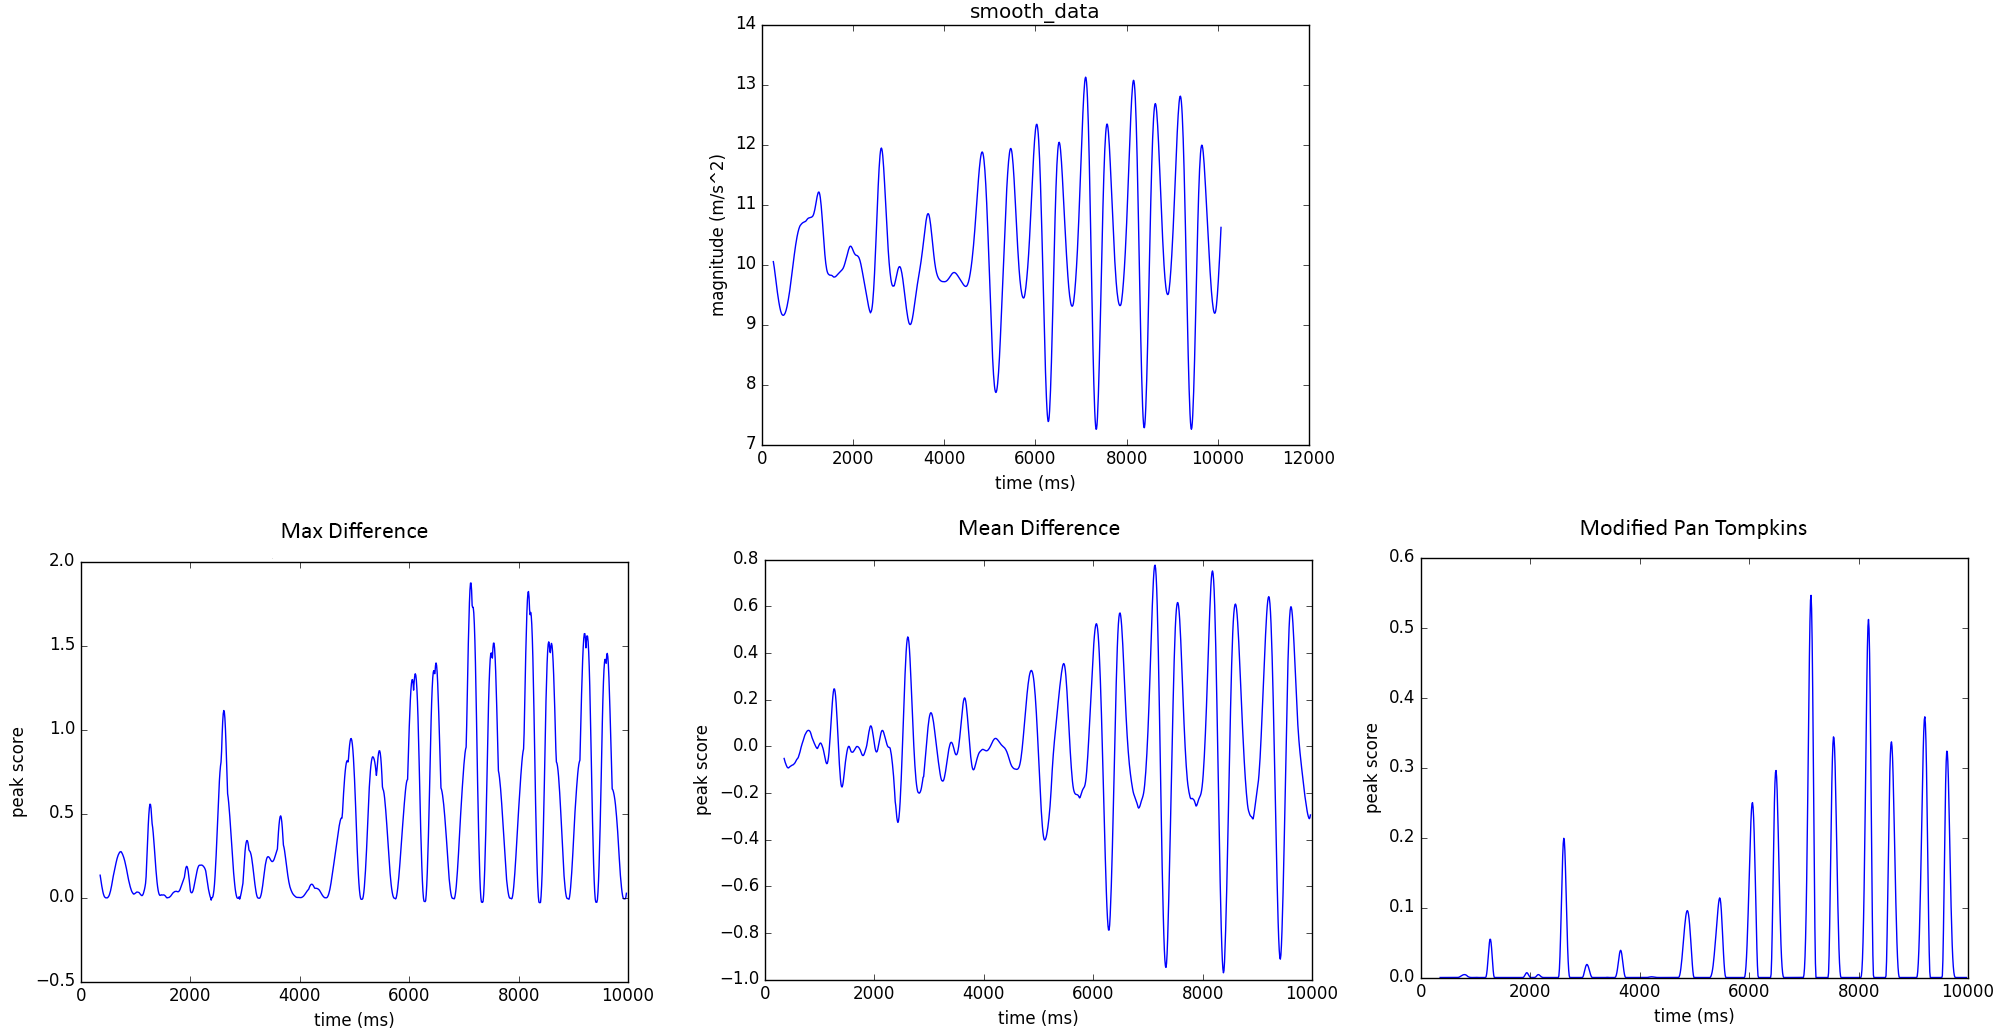
\includegraphics[width=\textwidth]{Images/compare_scoring.png}
                    \centering
                    \caption{Comparison of the three scoring methods on the same filtered signal. From left to right: Maximum Difference with $N=6$, Mean Difference with $N=10$, and Modified Pan-Tompkins with $N=10$.}
                    \label{img_compare_scoring}
                \end{figure}


        \section{Detection Stage}

            The next stage in the process is to identify potential candidates for peaks associated with steps. This is done using statistics to identify outliers. 

            As the algorithm processes the signal, it keeps track of a running mean and standard deviation. A computationally efficient way of doing this incrementally is as shown below:

            \begin{equation}
                \bar{x}_n = \frac{x_n + (n-1)\bar{x}_{n-1}}{n},
            \end{equation}

            \begin{equation}
                \sigma_n^2 = \frac
                {(n-2)\sigma_{n-1}^2 + (n-1)(\bar{x}_{n-1} -\bar{x}_n)^2 + (x - \bar{x}_n)^2}
                {n-1},
            \end{equation}

            where $x_n$ is the $n^{th}$ sample, $\bar{x}_n$ is the running mean at the $n^{th}$ sample, and $\sigma_n$ is the running standard deviation at the $n^{th}$ sample.

            The algorithm then uses these two quantities to determine whether any given point is an outlier by thresholding. If a point is more than $c$ current standard deviations above the current mean, then it is marked as a potential peak associated with a step, i.e. - if it satisfies the equation below:

            \begin{equation}
                \frac{x_n - \bar{x}_n}{\sigma_n}\geq c,
            \end{equation}

            where $c$ is the designated threshold.

            An example of the results from this method is shown below in Figure \ref{img_detection_stage}.

            Note that the algorithm builds up a running mean and standard deviation after initialisation. This means that, the first peak it encounters will be marked as a potential step.

            \begin{figure}[!th]
                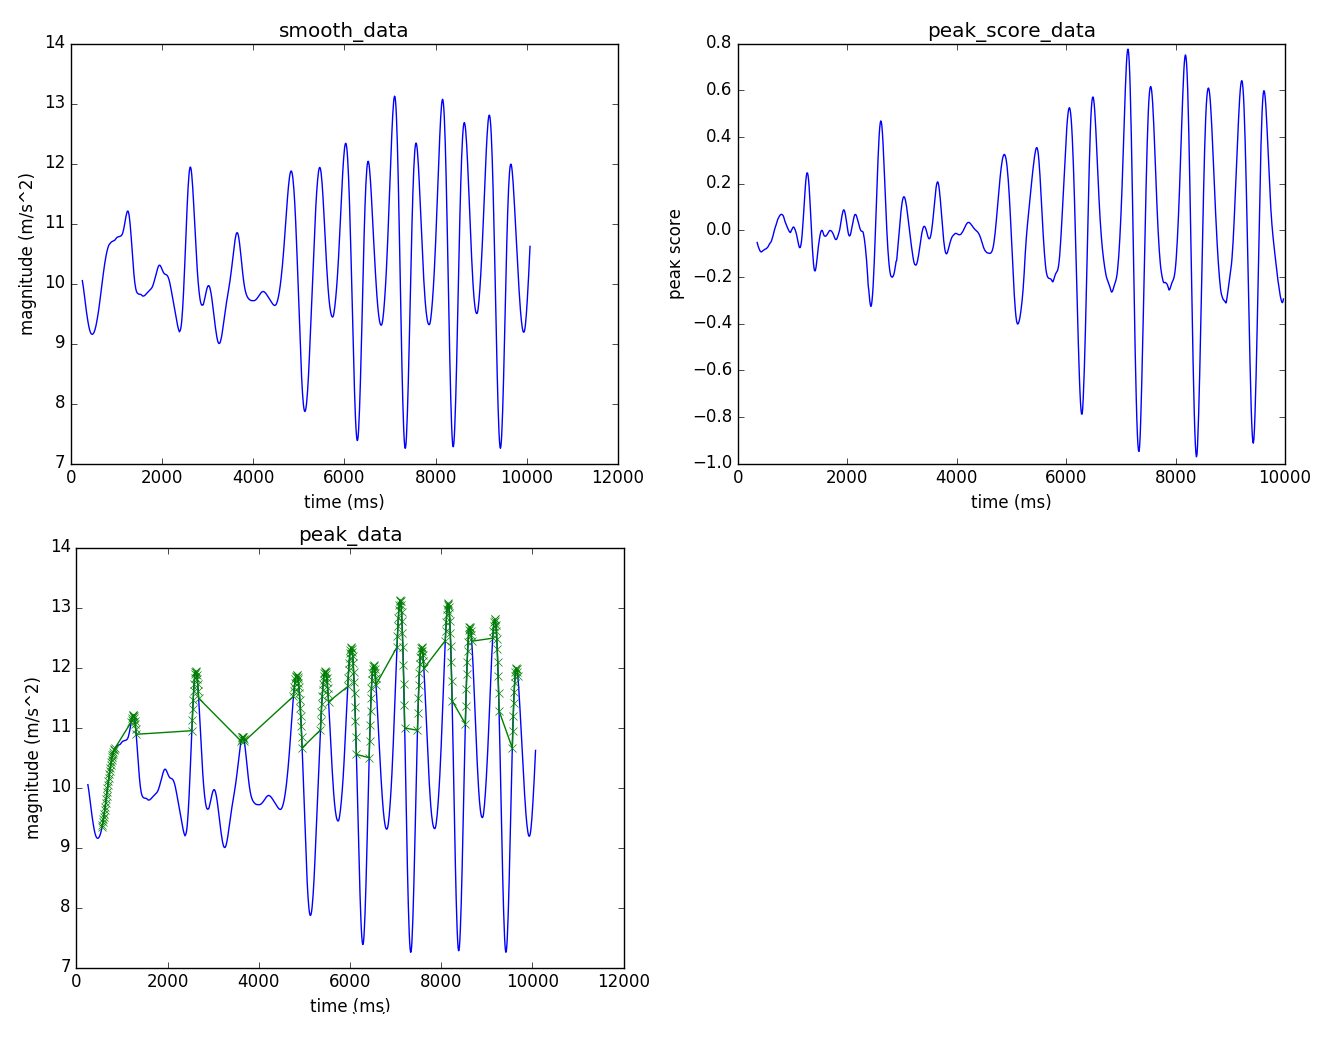
\includegraphics[width=\textwidth]{Images/detection_stage.png}
                \centering
                \caption{The results of the Peak Detection stage. Top Left: filtered signal, Top-Right: scored signal, Bottom-Left: filtered signal with potential peaks overlaid in green. $c=1.2$ for the Peak Detection stage.}
                \label{img_detection_stage}
            \end{figure}

        \section{Post-Processing Stage}

            The final stage of the algorithm is to identify the true peaks from the potential peaks from the previous stage. In Figure \ref{img_detection_stage}, all of the potential peak points are clustered on the rise to the main peak, This stage removes the erroneous points and leaves only the local maximum or the true peak. This stage also makes use of the fact that the peaks associated with walking are usually periodic with a minimum delay between them. Note this delay is related to the speed of walking.

            This stage slides a window of a fixed size, $t_{window}$, across the potential peaks and only keeps the maximum point within the window. This effectively removes all the points leading up to the peak while preserving the peak. By tuning the window size, the algorithm can ensure that for most cases no two steps will reside in this window at the same time. The window length was set to $200ms$ which corresponds to a maximum walking speed of $5 steps/sec$, much faster than average walking pace.

            The pseudocode for this step is as follows:

            \begin{lstlisting}
int windowSize = 200; // In ms
Point currentMax;
// Iterate through the sorted list of points
for (Point candidate in points) {
    if (candidate.time - currentMax.time > windowSize) {
        // The currentMax point is now outside the window. 
        yield currentMax;
        currentMax = candidate;
    } else {
        // Keep the maximum point.
        currentMax = (currentMax.value > candidate.value) ? currentMax : candidate;
    }
}
            \end{lstlisting}

            The result of this stage retains the main peak points while throwing away the points surrounding the peak, as intended. An example of this can be seen in \ref{img_post_stage}.

            \begin{figure}[!th]
                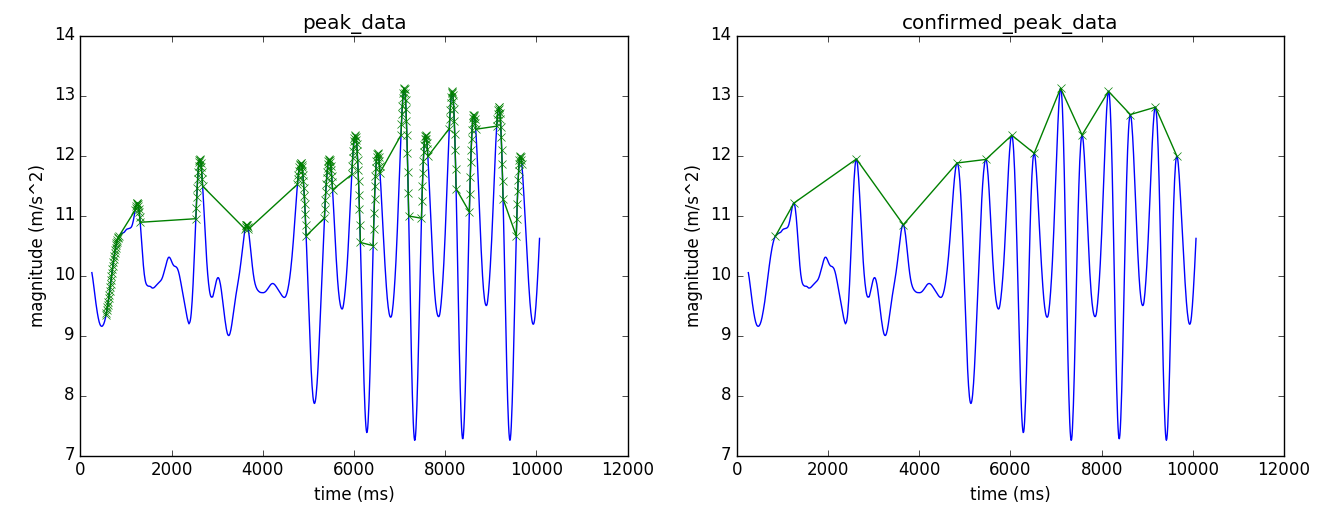
\includegraphics[width=\textwidth]{Images/post_stage.png}
                \centering
                \caption{The results of the Post-Processing Stage. Output of the Detection Stage is on the left, output of the Post-Processing Stage is on the right. Note how the set of points surrounding the peaks have been filtered out.}
                \label{img_post_stage}
            \end{figure}

    \chapter{Data Collection Equipment}
    \label{sc_device}

        A dataset with ground truth data must be acquired in order to optimize and validate the step-counting algorithm. The main goal is step counting over time, with the total count of steps being all that is required. However, in order to open up the versatility of the dataset and enable future improvements of the algorithm, a dataset was collected that would also contain the information for identifying the steps using reference data. Note that the total count of steps can easily be obtained from this more detailed dataset. 

        Previous studies, such as \cite{brajdic}, used video annotation to determine the time stamps of steps, but this is time intensive and prone to error. Instead, a custom device was designed and built to derive this information.

        \section{Design}

            The gold-standard device is designed to record steps with a sensor attached to the shoe. The sensors are connected to an RFduino, which is a Bluetooth-enabled Arduino microcontroller board. The RFduino polls the sensor for information and broadcasts it over Bluetooth Low Energy to an Android smartphone, as discussed later. 

            A first iteration of the device used push buttons mounted on straps as shown in Figure \ref{img_device_og_use}. These push buttons are connected to the RFduino with a simple pull-down resistor, such that logic level 0 indicates that the push button is up and the user's foot is up and logic level 1 indicates that the push button is down and the user's foot is down. A picture of the push button mounted on the straps can be seen below in Figure \ref{img_device_og}.

            \begin{figure}[!th]
                \includegraphics[width=0.6\textwidth]{Images/device_og.jpg}
                \centering
                \caption{A picture of the original ground truth device design. Note the push button in the middle of the pink strap. The contact area was reinforced with cardboard in an attempt to increase robustness.}
                \label{img_device_og}
            \end{figure}

            \begin{figure}[!th]
                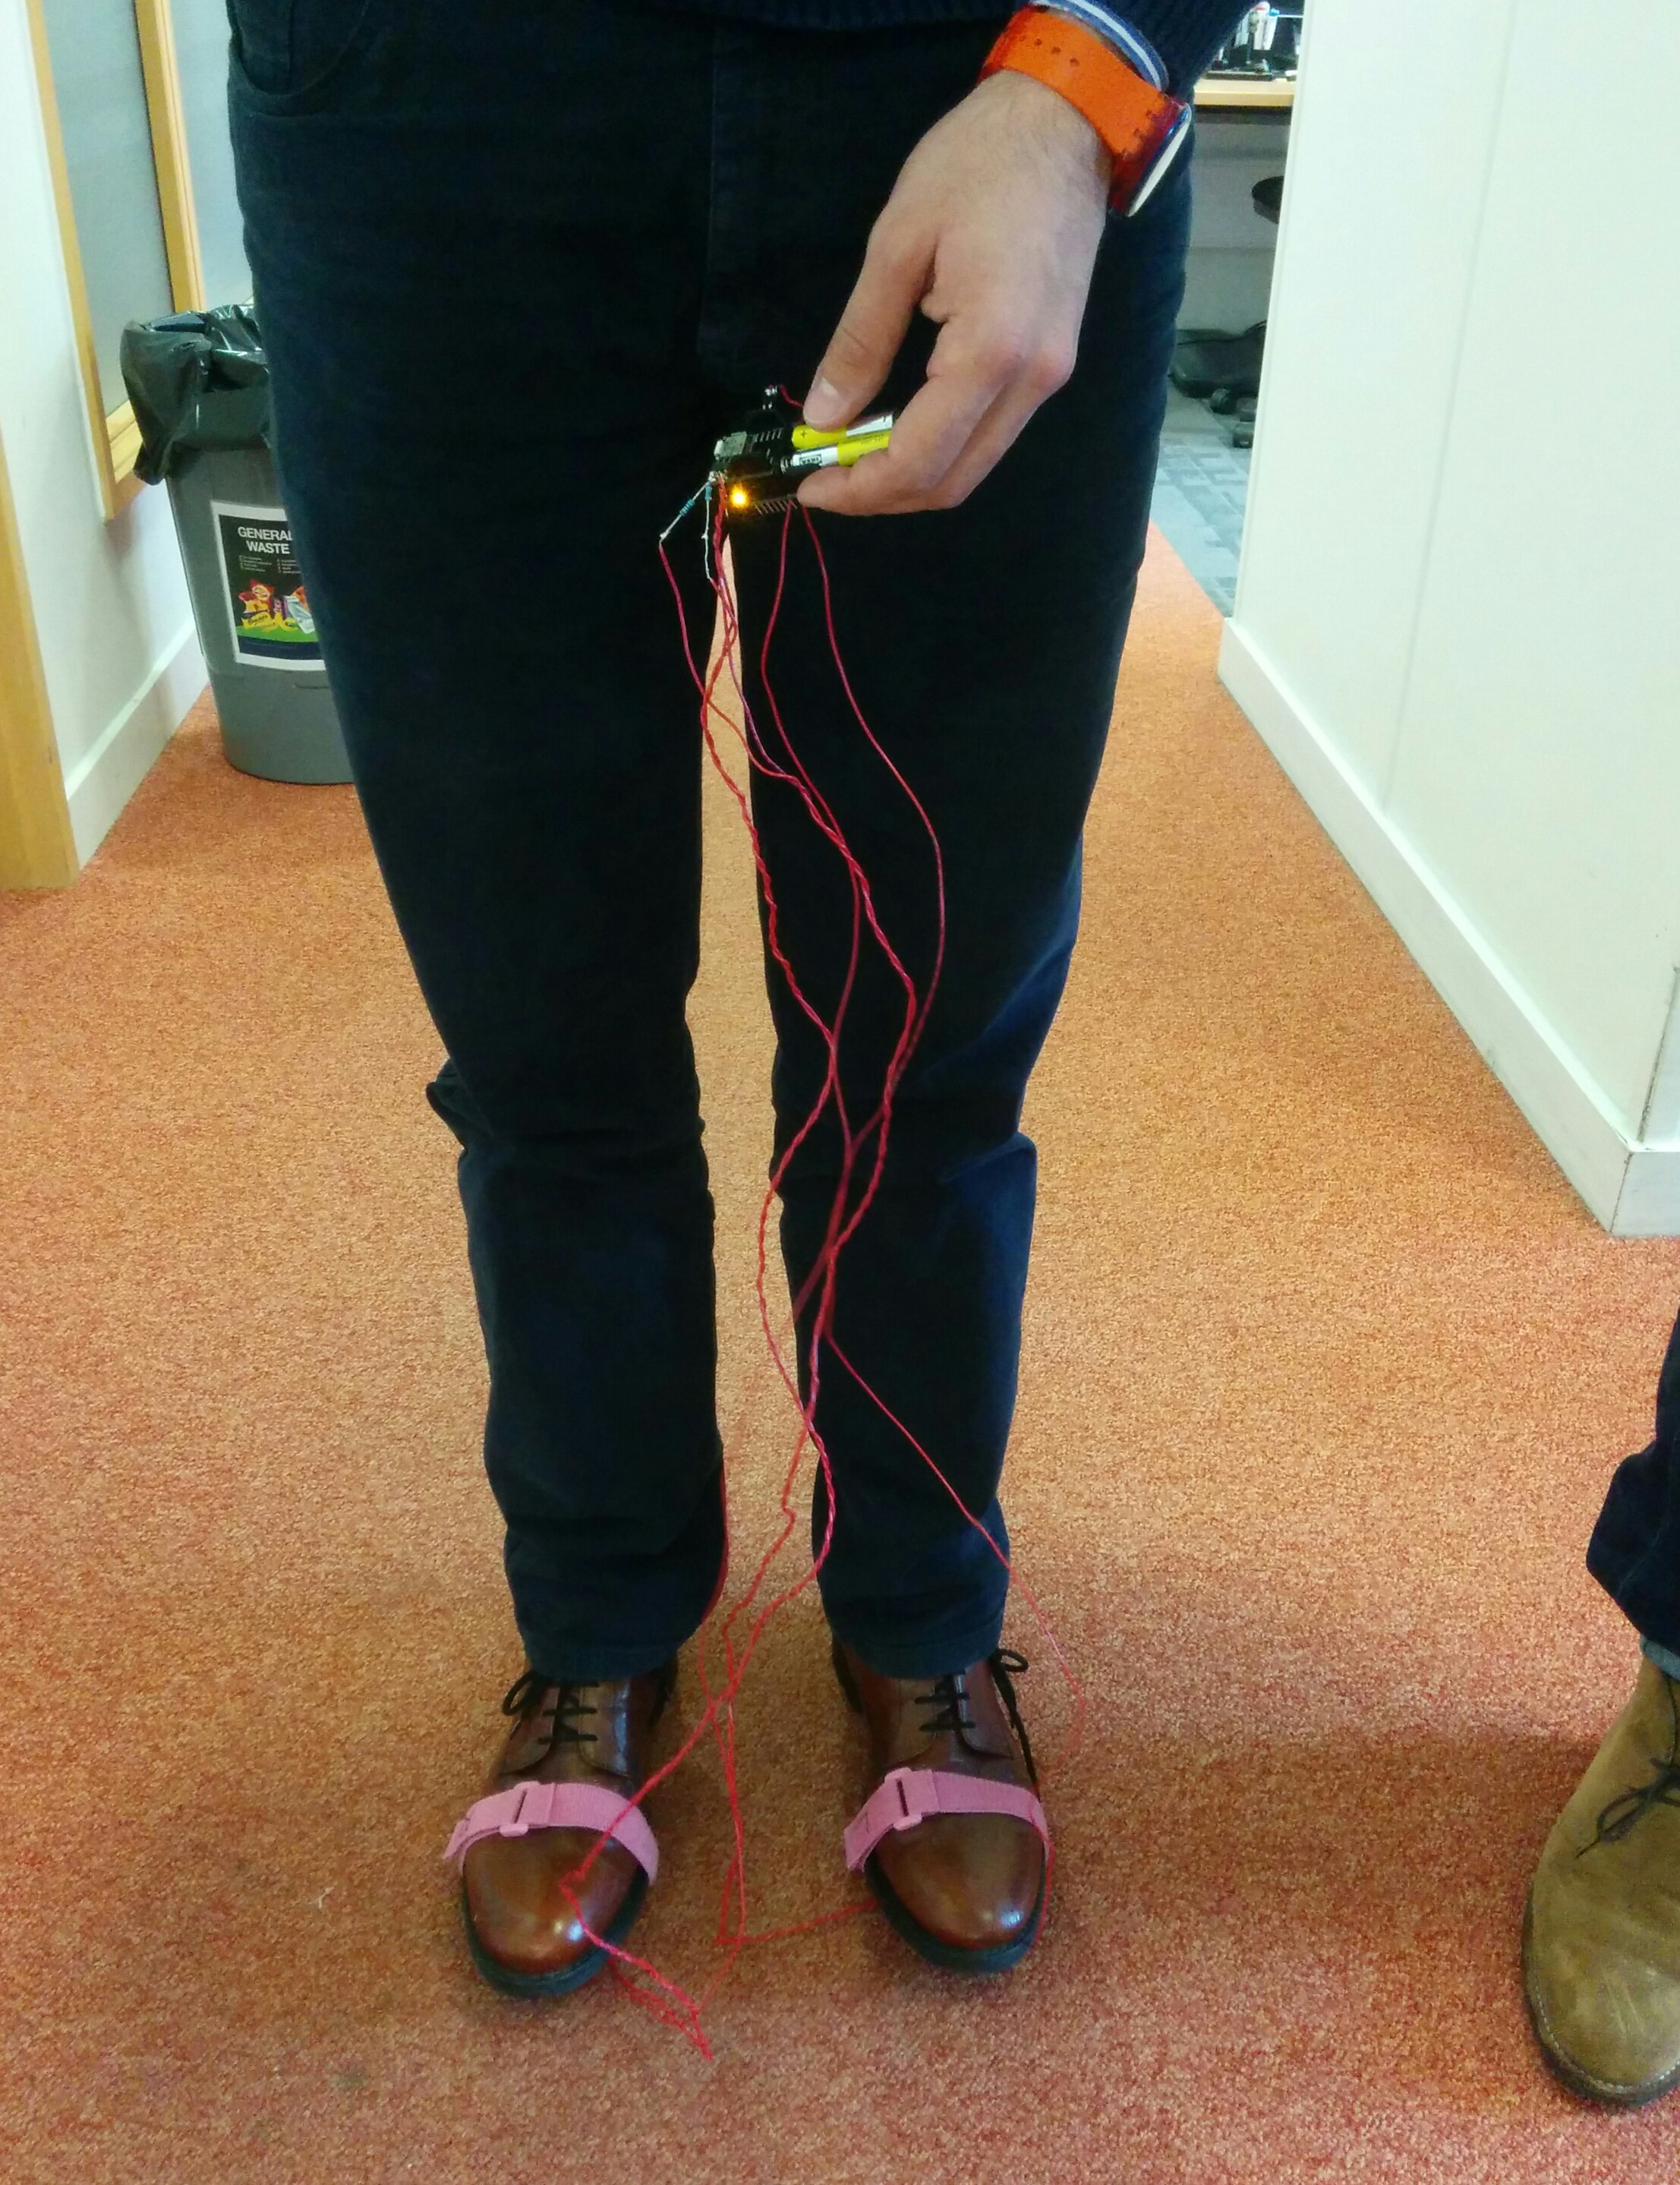
\includegraphics[width=0.6\textwidth]{Images/device_og_use.jpg}
                \centering
                \caption{A picture of the original ground truth device in use. Notice the placement of the straps on the user's shoes such that the push button is positioned roughly under the ball of the foot.}
                \label{img_device_og_use}
            \end{figure}

            Unfortunately, this first iteration of the device suffered from low robustness. The device was accurate when functional, but the push buttons broke due to excessive force. The pins of the push buttons also broke a number of times as they were folded flat against the strap due to the weight of the user.

            The second iteration of the design abandoned the push buttons entirely and relied instead on having a pressure-sensitive resistor positioned under the heel of the user inside the shoe. To ensure that this resistor was tolerant and sensitive to the relatively high pressures in this use case, the device used a material called velostat as the variable resistor. Velostat, used primiarly as a packaging material, is "made of polymeric foil impregnated with carbon black to make it electrically conductive" \cite{velostat}. The resistance is reduced when pressure is applied, hence a high current flow corresponds to the foot being down on the ground. The new device was made by taping conductive thread to either side of the velostat, completing the circuit. A picture of the new device can be seen in Figure \ref{img_device_new}.

            \begin{figure}[!th]
                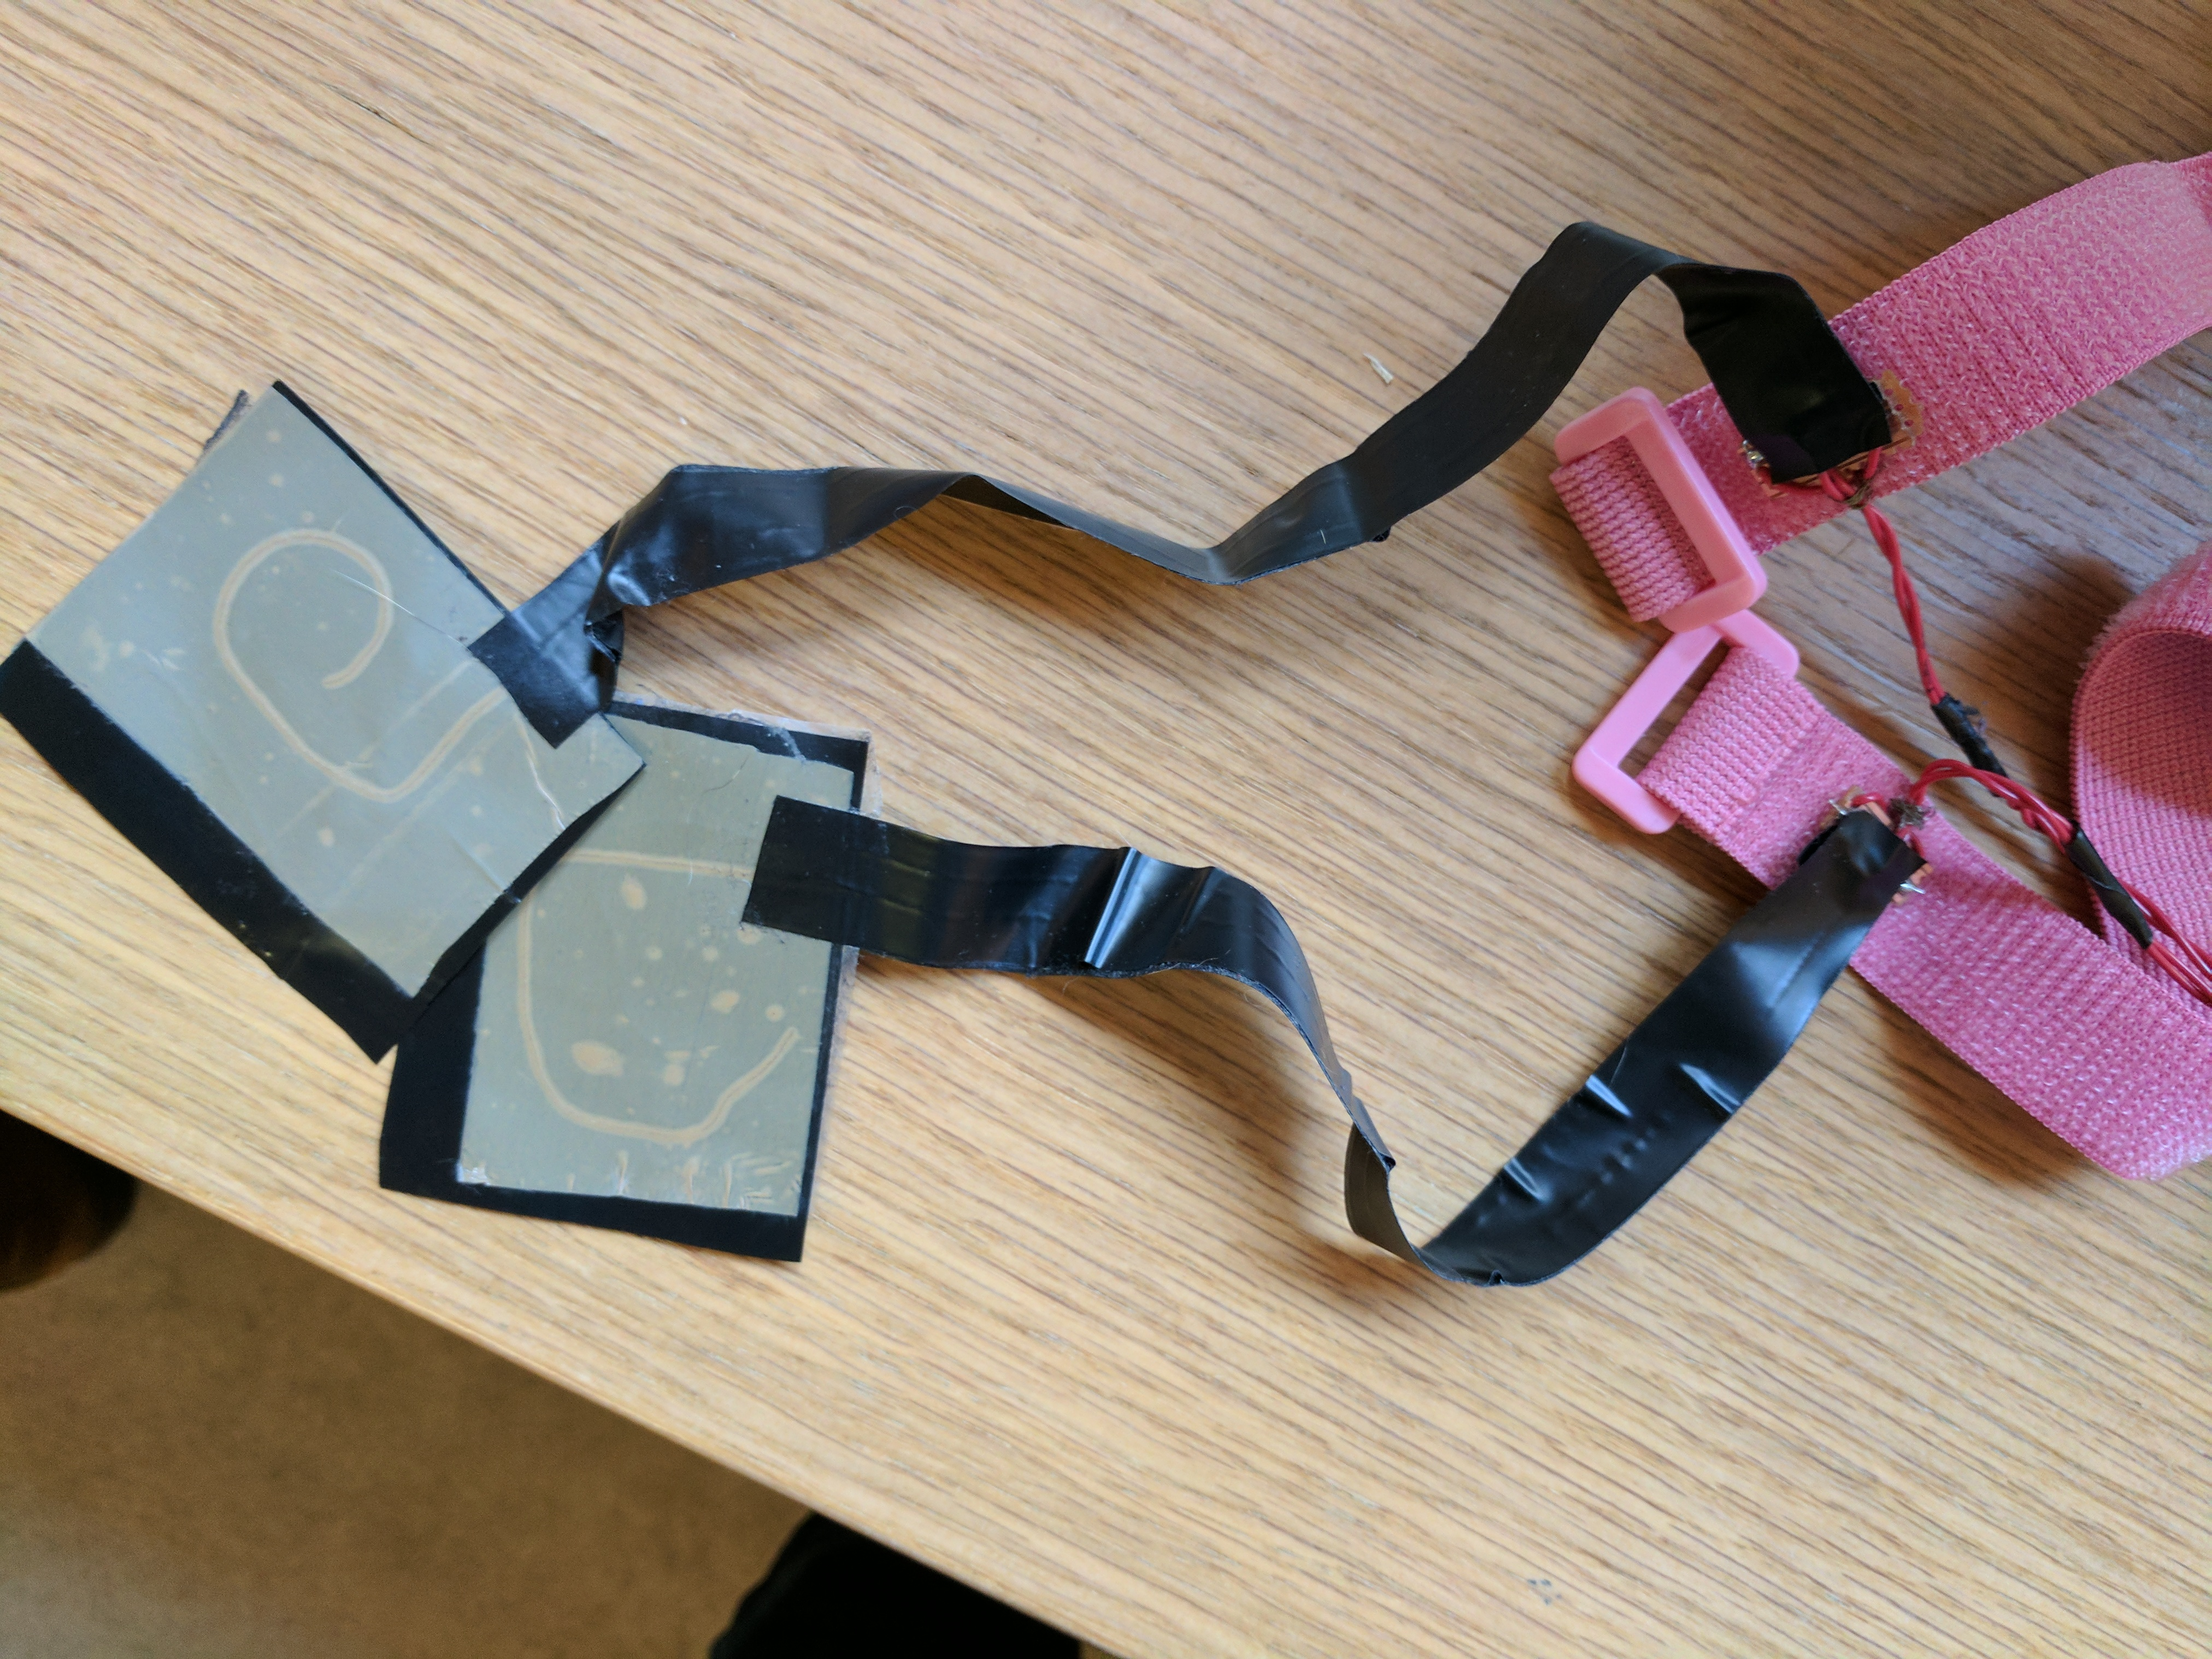
\includegraphics[width=0.6\textwidth]{Images/device_new.jpg}
                \centering
                \caption{The new ground truth device. Note the conductive thread visible through the tape and the electrical tape used to keep the two threads electrical isolated. The straps would now be put around the user's ankles.}
                \label{img_device_new}
            \end{figure}

            The firmware on the RFduino uses a moving threshold to determine the transition between the two states. The threshold for each sensor is updated by retaining the minimum and maximum values. Every 5 seconds, if the difference between these two exceeds a set minimum difference, the minimum and maximum are penalised by a factor proportional to the difference and the threshold is set to the midpoint between the minimum and maximum. This penalisation technique ensures that the minimum and maximum are local as minimum and maximum values that were set long ago would be penalised until a local value becomes relevant. A graph representing the raw data from the sensors plotted together with the thresholds against time is shown below in Figure \ref{img_device_new_graph}.

            \begin{figure}[!th]
                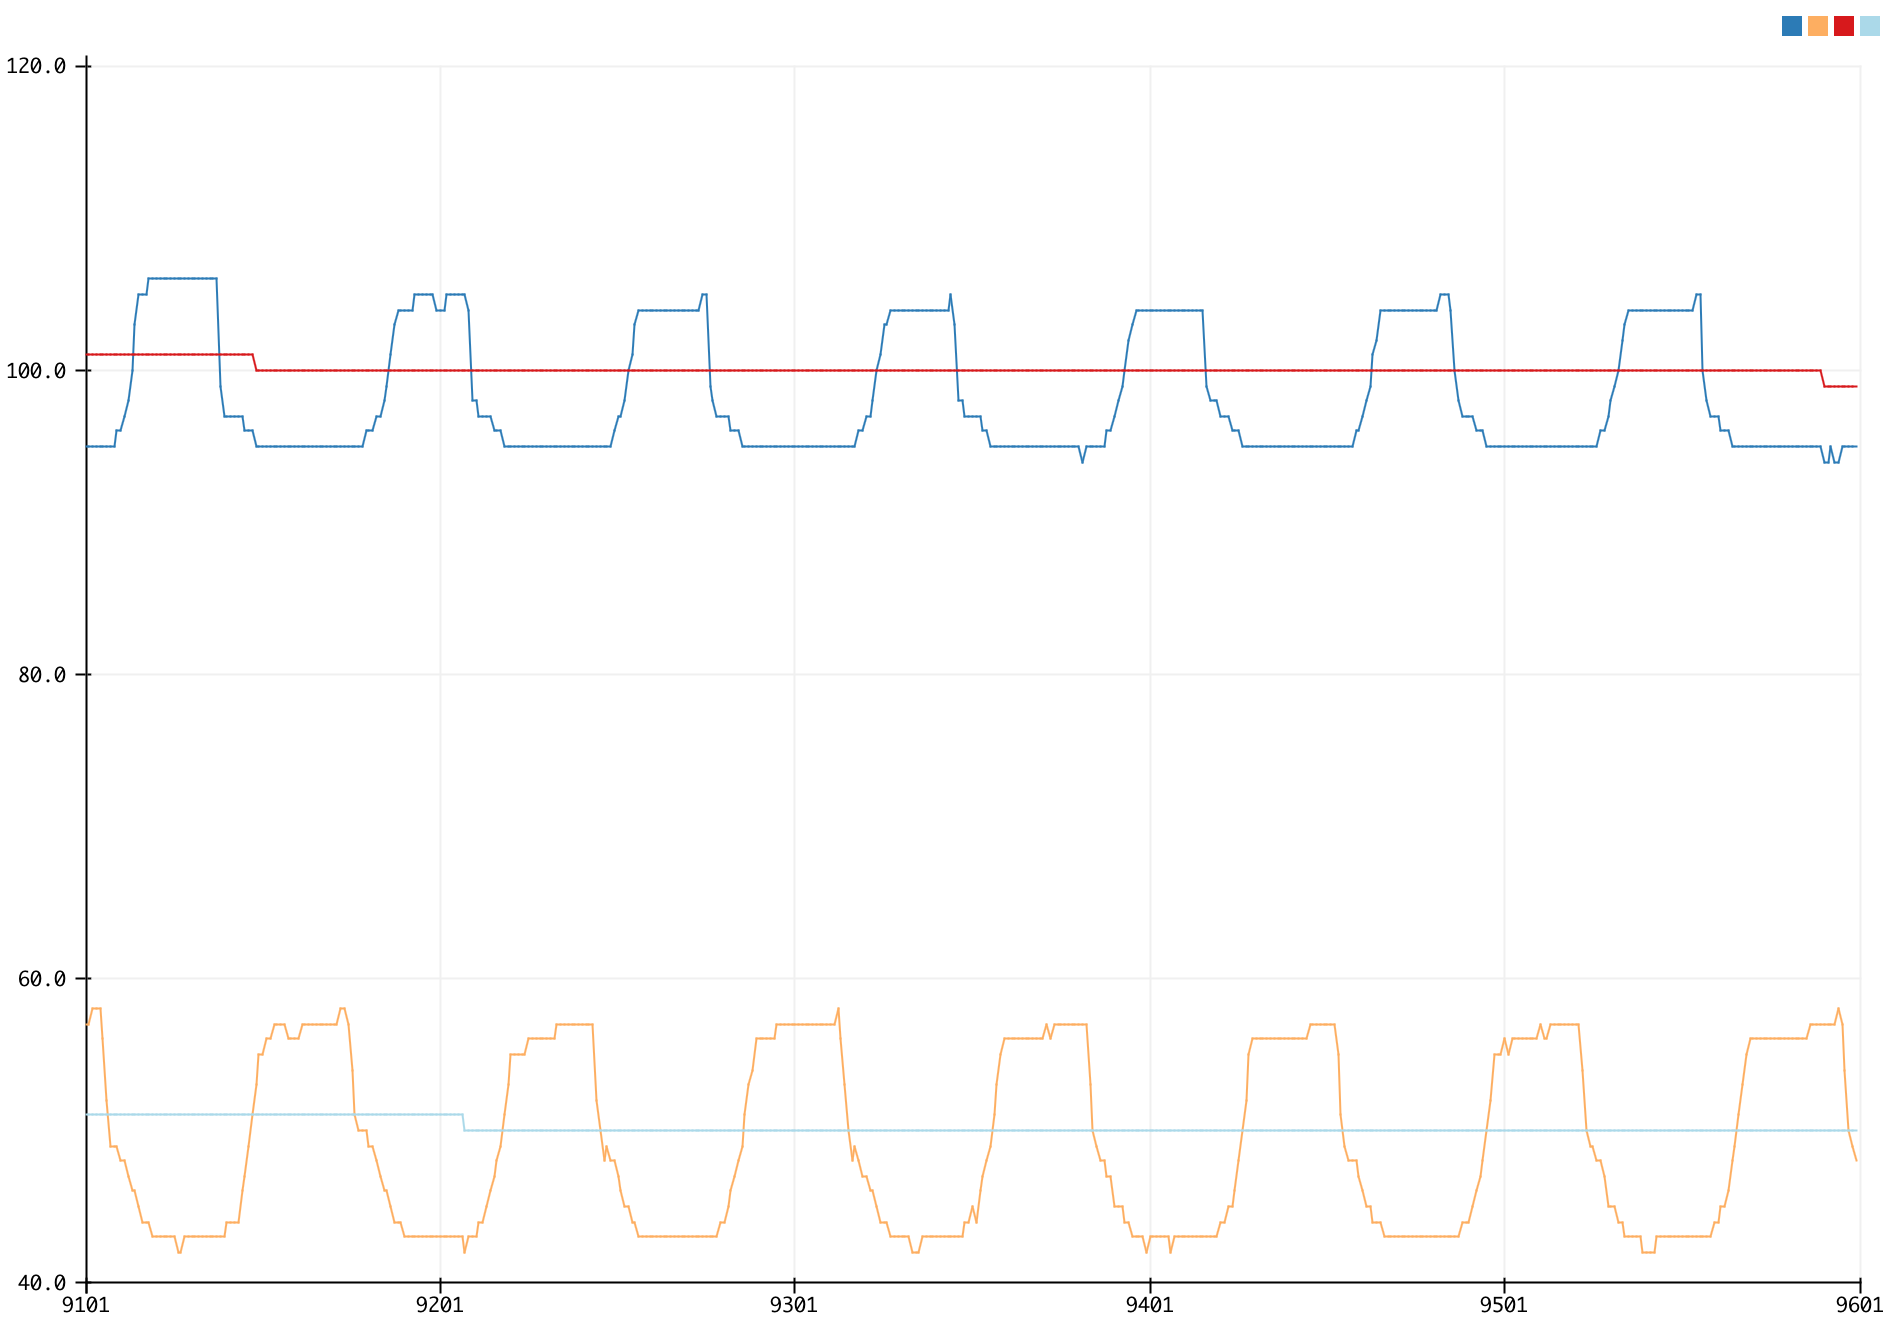
\includegraphics[width=0.8\textwidth]{Images/device_new_graph.png}
                \centering
                \caption{The raw data captured by the new ground truth device. Note how the steps are clearly discernable and the moving threshold correctly differentiates the two states. The difference in magnitude between the left-foot and right-foot signal is explained by the natural variation in velostat pads.}
                \label{img_device_new_graph}
            \end{figure}         


        \section{Android Application}

            To capture the accelerometer data and the ground truth simultaneously, an Android application had to be written to accommodate this functionality. The specifications were:

            \begin{itemize}
                \item Capture accelerometer data at a high sample rate (at least 100Hz) and save to a file.
                \item Connect via Bluetooth Low Energy to the ground-truth device, decode the signal, and save the data to a file with synchronized timestamps with respect to the accelerometer data.
                \item Provide a simple method of retrieving this data off the device.
                \item Provide a simple UI for the user to capture all of this data efficiently.
            \end{itemize}

            The application was designed such that the data would be zipped and compressed together and uploaded to a remote server via HTTP POST. This enabled the user to record multiple data recordings after one another without needing to manually retrieve the files off the device.


        \section{Data Collection}

            A dataset was collected that aimed to capture as many scenarios as possible. The dataset features three participants with different of heights and weights, 3 smartphones (a Google Pixel, a Samsung Galaxy S6, and a Google Nexus 5 device) to ensure that similar devices performed similarly, and 6 phone 'positions': in a hand, in a front pocket, in a back pocket, in an armband, in a shoulder purse, and in a neck pouch on a lanyard. In order to ensure generality, recordings were made on two different surfaces: hard floor (stone or linoleum) and carpeted floors. This resulted in a dataset containing 48 distinct recordings, each with approximately $2.5$ minutes of accelerometer and ground-truth data. 

            In addition, 3 recordings were collected from consenting patients participating in a clinical pilot study without the ground truth device data for post-optimization validation. The total steps, in these 3 instances, were hand counted by a trained healthcare professional present at the recording.

    \chapter{Algorithm Optimization}

         Optimization of the algorithm can be described as a maximization problem for which the problem domain is defined by the parameter space. The only way of getting a close to the true maximum is to run an exhaustive grid search across the parameter space. Each stage may have parameters associated with it, and these parameters may change depending on the stage selection (choice of filter, scoring technique). 

        For the running time of the optimization routine to be kept within a reasonable limits, the parameter search will need to be fairly coarse to limit the number of parameter permutations. The final set can be seen in Tables \ref{tbl_filtering}, \ref{tbl_scoring}, \ref{tbl_detection}. Note that the first stage, Pre-Processing, has been held constant at $t_{scale}=10^6$ and $f_{int}=100Hz$. The Post-Processing stage has also been held constant at $t_{window}=200ms$. 


        \begin{center}
            \captionof{table}{The parameter set for the Filtering Stage.}
            \label{tbl_filtering}
            \begin{tabular}{|c|c|c|c|}
                \hline
                Parameter & Minimum & Step & Maximum \\
                \hline
                \multicolumn{4}{|c|}{\textbf{Moving Average Filter}} \\
                \hline
                Window Size ($N$) & 13 & 8 & 53 \\
                \hline
                \multicolumn{4}{|c|}{\textbf{Hann Filter}} \\
                \hline
                Window Size ($N$) & 13 & 8 & 53 \\
                \hline
                \multicolumn{4}{|c|}{\textbf{Gaussian Filter}} \\
                \hline
                Window Size ($N$) & 13 & 8 & 53 \\
                Standard Deviation ($\sigma$) & 0.35 & Fixed & 0.35 \\
                \hline
                \multicolumn{4}{|c|}{\textbf{Kaiser-Bessel Filter}} \\
                \hline
                Window Size ($N$) & 13 & 8 & 53 \\
                Sampling Frequency ($f_s$) & 100Hz & Fixed & 100Hz \\
                Cutoff Frequency ($f_c$) & 3Hz & Fixed & 3Hz \\
                Drop At $f_c$ ($A$) & 60dB & Fixed & 60dB \\
                \hline
            \end{tabular}
        \end{center}

        \begin{center}
            \captionof{table}{The parameter set for the Scoring Stage.}
            \label{tbl_scoring}
            \begin{tabular}{|c|c|c|c|}
                \hline
                Parameter & Minimum & Step & Maximum \\
                \hline
                \multicolumn{4}{|c|}{\textbf{Maximum Difference}} \\
                \hline
                Window Size ($N$) & 3 & 8 & 51 \\
                \hline
                \multicolumn{4}{|c|}{\textbf{Mean Difference}} \\
                \hline
                Window Size ($N$) & 3 & 8 & 51 \\
                \hline
                \multicolumn{4}{|c|}{\textbf{Modified Pan Tompkins}} \\
                \hline
                Window Size ($N$) & 11 & 8 & 51 \\
                \hline
                \multicolumn{4}{|c|}{\textbf{No Scoring Method}} \\
                \hline
                \multicolumn{4}{|c|}{No Parameters} \\
                \hline
            \end{tabular}
        \end{center}
        \begin{center}
            \captionof{table}{The parameter set for the Detection Stage.}
            \label{tbl_detection}
            \begin{tabular}{|c|c|c|c|}
                \hline
                Parameter & Minimum & Step & Maximum \\
                \hline
                Standard Deviation Threshold ($c$) & 1.2 & 0.2 & 1.4 \\
                \hline
            \end{tabular}
        \end{center}

        These parameter variations give a total number of permutations equal to 1008. Each of these parameter sets was tested on all 48 data recordings listed in the previous section. The results were averaged across all data recordings for each permutation to give an overall value for the accuracy.

        However, since there are approximately $2$ hours of data to run through the algorithm, each combination of parameters takes 5 minutes to be tested on a machine with an Intel i5-6200u. If the optimization were run solely on that machine, it would take $3.5$ days to complete.

        The solution to this problem was to build a distributed computing platform such that the computing load could be spread across multiple machines. The backend server was built on Flask \cite{flask}, a web microframework for Python, and served over gunicorn \cite{gunicorn}, a Python WSGI (Web Server Gateway Interface) HTTP webserver. The data was passed back and forward via JSON (JavaScript Object Notation). The backend would also store the results in a PostgreSQL (Structured Query Language) database \cite{postgres} such that the results could be queried easily.

        Each machine had a local implementation of the algorithm and a copy of the dataset. The machine queried the backend for a new set of parameters, and fetched the JSON of these with an HTTP GET request. Once the computation was completed, the machine appended the results to the JSON file and returned it via an HTTP POST request to the backend. A new set of parameters was then requested, until all permutations had been exhausted.

        In this instance, Google Cloud Compute \cite{gcc} was used to instantiate 8 machines to run the algorithm, such that the runtime for the exhaustive search was cut down to around 11 hours.

    \chapter{Results}

        Note that in the following chapter, all of the statistics given are in terms of accuracy defined by:

        \begin{equation}
            a = 100(1 - \frac{|s_{a}-s_{gt}|}{s_{gt}}),
        \end{equation}

        where $a$ is the accuracy, $s_{a}$ is the number of steps from the algorithm and $s_{gt}$ is the number of steps in the ground truth.

        \section{Variability in Surface and Phone}

            Our first investigation is concerned with the differences between floor surfaces and phone devices. 

            \subsection{Variability Surface}

                There are 4 recordings from the Google Pixel on each of the surfaces listed: hard (stone or linoleum) and carpet. All of these recordings were carried out with the phone in hand. To check the variation between these surfaces, the algorithm parameters are held constant and the average score is checked for each surface. The results of these tests can be seen below in Table \ref{tbl_surface_results}. Note that the parameters used were those of the optimal set, as detailed in the next section.

                \begin{center}
                    \captionof{table}{The results for each of the recordings according to surface.}
                    \label{tbl_surface_results}
                    \begin{tabular}{|c|c|c|c|}
                        \hline
                        Recording & Ground Truth (steps) & Algorithm Output (steps) & Accuracy \\
                        \hline
                        \multicolumn{4}{|c|}{\textbf{Hard Floor}} \\
                        \hline
                        1 & 292 & 298 & 97.9\% \\
                        2 & 267 & 271 & 98.1\% \\
                        3 & 323 & 290 & 89.7\% \\
                        4 & 322 & 307 & 95.3\% \\
                        \hline
                        Average & - & - & 95.3\% \\
                        \hline
                        \multicolumn{4}{|c|}{\textbf{Carpet}} \\                        
                        \hline
                        1 & 243 & 245 & 99.1\% \\
                        2 & 255 & 263 & 96.9\% \\
                        3 & 206 & 246 & 80.6\% \\
                        4 & 195 & 257 & 68.2\% \\
                        \hline
                        Average & - & - & 86.2\% \\
                        \hline
                    \end{tabular}
                \end{center}

                While there is a noticeable difference between the accuracies obtained on hard floor versus carpet, the high variance in the carpet results means that it is not possible to tell whether there is a meaningful difference between the types of surfaces or whether Carpet Recording 4, which lowered the average significantly was an isolated instance. Further tests would be needed to be recorded to confirm this hypothesis.

            \subsection{Phone}

                The difference between phones is expected to be negligible and this proved to be the case. These data recordings were taken with each phone: Google Pixel, Google Nexus 5, and Samsung S6. The phone was held in hand and the surface was a hard floor. As with the analysis for the different surfaces, the algorithm parameters were those of the optimal set as described below. The table of results is shown below in Table \ref{tbl_phone_results}

                \begin{center}
                    \captionof{table}{The results for each of the recordings according to the phone. Note that only 2 recordings were made with each of the Google Nexus 5 and Samsung S6.}
                    \label{tbl_phone_results}
                    \begin{tabular}{|c|c|c|c|}
                        \hline
                        Recording & Ground Truth (steps) & Algorithm Output (steps) & Accuracy \\
                        \hline
                        \multicolumn{4}{|c|}{\textbf{Google Pixel}} \\
                        \hline
                        1 & 292 & 298 & 97.9\% \\
                        2 & 267 & 271 & 98.1\% \\
                        3 & 323 & 290 & 89.7\% \\
                        4 & 322 & 307 & 95.3\% \\
                        \hline
                        Average & - & - & 95.3\% \\
                        \hline
                        \multicolumn{4}{|c|}{\textbf{Google Nexus 5}} \\                        
                        \hline
                        1 & 305 & 293 & 96.1\% \\
                        2 & 306 & 298 & 97.3\% \\
                        \hline
                        Average & - & - & 96.8\%\\
                        \hline
                        \multicolumn{4}{|c|}{\textbf{Samsung S6}} \\                        
                        \hline
                        1 & 266 & 265 & 99.6\% \\
                        2 & 265 & 253 & 95.5\% \\
                        \hline
                        Average & - & - & 97.6\% \\
                        \hline
                    \end{tabular}
                \end{center}

                By inspection, it is clear that the choice of phone has no significant impact on accuracy.           

        \section{Optimal Parameters}

            With the optimal set of parameters, an average accuracy of 93.7\% and a median accuracy of 96.8\% are obtained across the 48 data recordings. The parameters that achieve this accuracy are given by Table \ref{tbl_opt_params}.

            \begin{center}
                \captionof{table}{The parameters for the optimal algorithm performance.}
                \label{tbl_opt_params}
                \begin{tabular}{|c|c|c|}
                    \hline
                    Stage & Type & Parameters \\
                    \hline
                    Pre-Processing & Default & $t_{scale}=10^6$, $f_{int}=100Hz$ \\
                    Filtering & Gaussian & $N=13$, $\sigma=0.35$ \\
                    Scoring & Mean Difference & $N=27$ \\
                    Detection & Default & $c=1.2$ \\
                    Post-Processing & Default & $t_{window}=200ms$ \\
                    \hline
                \end{tabular}
            \end{center}

            The spread of the accuracy results can be seen below in Figure \ref{img_opt_params_overall}. This shows that the majority of the accuracy results is within the 90\% to 100\% range with some outliers showing significantly lower accuracy.

            \begin{figure}[!th]
                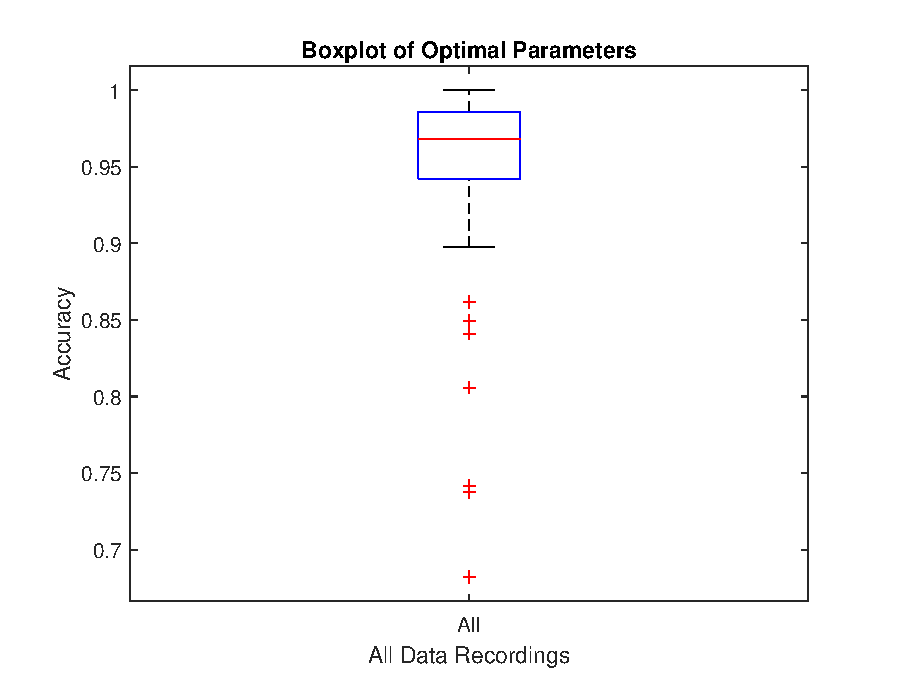
\includegraphics[width=0.8\textwidth]{Images/opt_params_overall.eps}
                \centering
                \caption{The spread of the accuracy of the optimal parameters over the 48 data recordings.}
                \label{img_opt_params_overall}
            \end{figure}

            If the results are split according to the position of the phone during the recordings, the source of these outliers becomes evident. These plots can be seen below in Figure \ref{img_opt_params_positions_bp}.

            \begin{figure}[!th]
                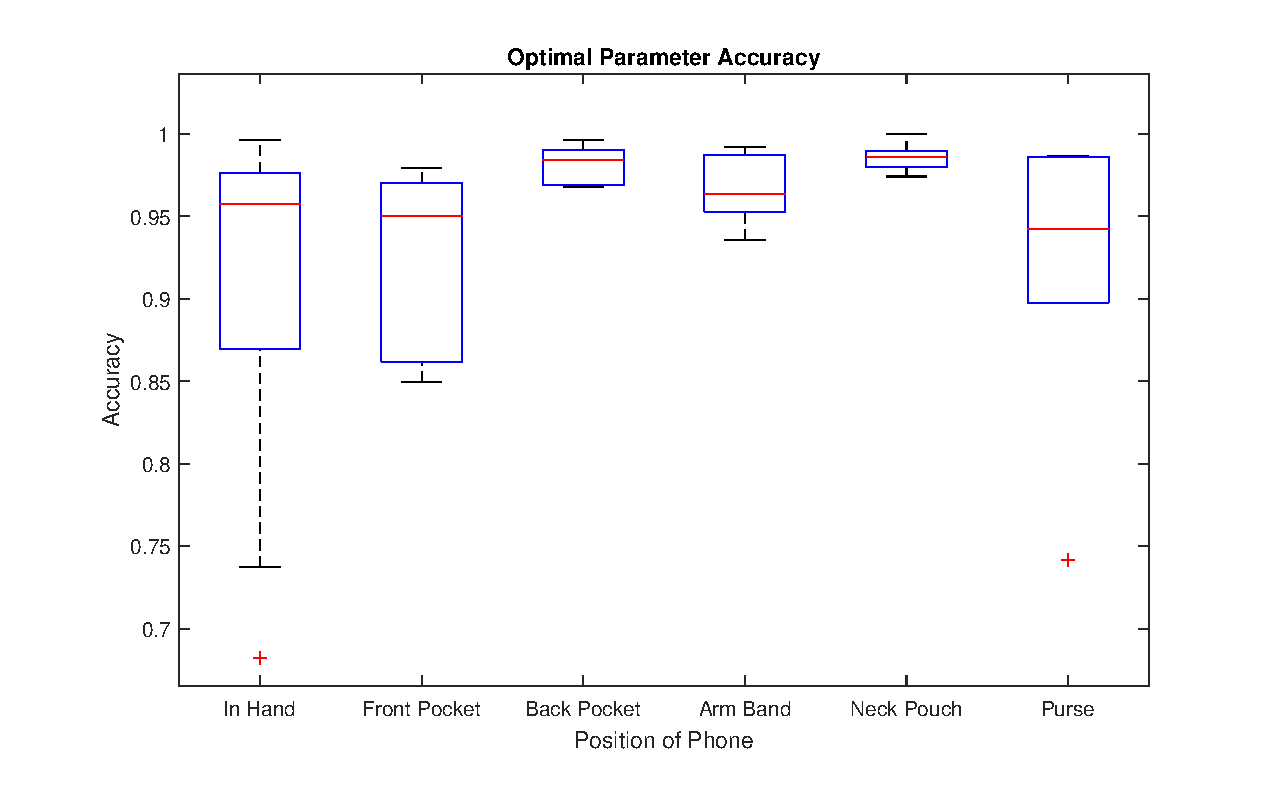
\includegraphics[width=0.8\textwidth]{Images/opt_params_positions_bp.eps}
                \centering
                \caption{The spread of the accuracy of the optimal parameters over the 48 data recordings grouped by phone position. The far outliers come from the 'In Hand' position.}
                \label{img_opt_params_positions_bp}
            \end{figure}

            As can be seen from Figure \ref{img_opt_params_positions_bp}, the outliers come primarily from the 'In Hand' or 'Purse' positions. This leads to the hypothesis that these positions may induce some harmonics in the walking frequency range. The source of these may be the user swinging their arm when holding the phone or the purse swinging back and forth under arm.

            This grouping also reveals that the 'Back Pocket', 'Arm Band', and 'Neck Pouch' positions seem to be the best positions. It should be noted that the 'Arm Band' may be subject to the same harmonics as the 'In Hand' position; however, the relatively limited movement of the upper arm when compared to the hand limits the impact of these harmonics.

            These parameters can now be validated against the three patient data recordings mentioned earlier. If the accuracies are similar to the average, then it supports the idea that these parameters are near optimal.

            The results of applying the algorithm with the optimal set of parameters to the patient recordings are detailed below in Table \ref{tbl_patient_results}. The average accuracy is 92.3\%. This is very close to the average accuracy obtained with the 48 data recordings used to optimise the algorithm and well within the median quartiles in the boxplot.

            \begin{center}
                \captionof{table}{The results of the optimal parameters for the three patient data recordings.}
                \label{tbl_patient_results}
                \begin{tabular}{|c|c|c|c|}
                    \hline
                    Label & Observed Number of Steps & Algorithm Output & Accuracy \\
                    \hline
                    Patient 1 & 614 & 654 & 93.5\% \\ 
                    Patient 2 & 567 & 605 & 93.2\% \\
                    Patient 3 & 682 & 749 & 90.2\% \\
                    \hline
                \end{tabular}
            \end{center}

        \section{Position Specific Parameters}

            The investigations above revealed a that a given set of parameters performs differently on different positions. This leads to the idea that the algorithm may be able to switch between parameters given the position of the phone to give the best result. For each position, a set of optimal parameters will be determined and then specified for that position. This analysis leads to very high accuracies for some positions.

            The optimal parameters for the In Hand, Front Pocket, Arm Band, Neck Pouch, and Purse positions all have the types of stage in common, so these will be reported together for brevity. The types of stage for the mentioned positions are: Moving Average for the Filtering Stage and Mean Difference for the Scoring Stage. For all of these, the Pre-Processing stage used $t_{scale} = 10^6$ and $f_{int} = 100Hz$ and the Post-Processing stage used $t_{window} = 200ms$. The rest of the parameters for these positions are given in Table \ref{tbl_params_bundle}.

            \begin{center}
                \captionof{table}{The parameters for the optimal algorithm performance in the In Hand, Front Pocket, Arm Band, Neck Pouch, and Purse position.}
                \label{tbl_params_bundle}
                \begin{tabular}{|c|c|c|c||c|}
                    \hline
                    Position & Filtering & Scoring & Detection & Average Accuracy \\
                    \hline
                    In Hand & $N=53$ & $N=11$ & $c=1.4$ & 92.4\% \\
                    Front Pocket & $N=29$ & $N=27$ & $c=1.2$ & 98.0\% \\
                    Arm Band & $N=21$ & $N=3$ & $c=1.2$ & 99.4\% \\
                    Neck Pouch & $N=21$ & $N=11$ & $c=1.2$ & 98.9\% \\
                    Purse & $N=29$ & $N=11$ & $c=1.2$ & 96.9\% \\
                    \hline
                \end{tabular}
            \end{center}  

            \subsection{Back Pocket}

                The best set of parameters for the 'Back Pocket' position gives an overall accuracy of 99.2\%. The parameters that achieve this are given in Table \ref{tbl_params_back_pocket}.

                \begin{center}
                    \captionof{table}{The parameters for the optimal algorithm performance in the 'Back Pocket' position.}
                    \label{tbl_params_back_pocket}
                    \begin{tabular}{|c|c|c|}
                        \hline
                        Stage & Type & Parameters \\
                        \hline
                        Pre-Processing & Default & $t_{scale}=10^6$, $f_{int}=100Hz$ \\
                        Filtering & Gaussian & $N=21$, $\sigma=0.35$ \\
                        Scoring & No Scoring & \\
                        Detection & Default & $c=1.2$ \\
                        Post-Processing & Default & $t_{window}=200ms$ \\
                        \hline
                    \end{tabular}
                \end{center}



    \chapter{Further Work}
        The impact of surface on the results shall be further investigated. A larger sample size is required to determine whether there is any significant difference in algorithm performance between different floor surfaces.

        Since the timestamps data for the actual steps data exists in the database, one direction of exploration could be to analyse how many steps the algorithm identifies correctly and how many steps the algorithm misses. This is equivalent to a false positive/false negative analysis.

        Another area that could be explored is a less coarse search for the optimal parameters. The results so far could be treated as being preliminary and a finer grained search over the parameter space could be run to yield the true maximum.